\documentclass[twoside]{book}

% Packages required by doxygen
\usepackage{fixltx2e}
\usepackage{calc}
\usepackage{doxygen}
\usepackage[export]{adjustbox} % also loads graphicx
\usepackage{graphicx}
\usepackage[utf8]{inputenc}
\usepackage{makeidx}
\usepackage{multicol}
\usepackage{multirow}
\PassOptionsToPackage{warn}{textcomp}
\usepackage{textcomp}
\usepackage[nointegrals]{wasysym}
\usepackage[table]{xcolor}

% Font selection
\usepackage[T1]{fontenc}
\usepackage[scaled=.90]{helvet}
\usepackage{courier}
\usepackage{amssymb}
\usepackage{sectsty}
\renewcommand{\familydefault}{\sfdefault}
\allsectionsfont{%
  \fontseries{bc}\selectfont%
  \color{darkgray}%
}
\renewcommand{\DoxyLabelFont}{%
  \fontseries{bc}\selectfont%
  \color{darkgray}%
}
\newcommand{\+}{\discretionary{\mbox{\scriptsize$\hookleftarrow$}}{}{}}

% Page & text layout
\usepackage{geometry}
\geometry{%
  a4paper,%
  top=2.5cm,%
  bottom=2.5cm,%
  left=2.5cm,%
  right=2.5cm%
}
\tolerance=750
\hfuzz=15pt
\hbadness=750
\setlength{\emergencystretch}{15pt}
\setlength{\parindent}{0cm}
\setlength{\parskip}{3ex plus 2ex minus 2ex}
\makeatletter
\renewcommand{\paragraph}{%
  \@startsection{paragraph}{4}{0ex}{-1.0ex}{1.0ex}{%
    \normalfont\normalsize\bfseries\SS@parafont%
  }%
}
\renewcommand{\subparagraph}{%
  \@startsection{subparagraph}{5}{0ex}{-1.0ex}{1.0ex}{%
    \normalfont\normalsize\bfseries\SS@subparafont%
  }%
}
\makeatother

% Headers & footers
\usepackage{fancyhdr}
\pagestyle{fancyplain}
\fancyhead[LE]{\fancyplain{}{\bfseries\thepage}}
\fancyhead[CE]{\fancyplain{}{}}
\fancyhead[RE]{\fancyplain{}{\bfseries\leftmark}}
\fancyhead[LO]{\fancyplain{}{\bfseries\rightmark}}
\fancyhead[CO]{\fancyplain{}{}}
\fancyhead[RO]{\fancyplain{}{\bfseries\thepage}}
\fancyfoot[LE]{\fancyplain{}{}}
\fancyfoot[CE]{\fancyplain{}{}}
\fancyfoot[RE]{\fancyplain{}{\bfseries\scriptsize Generated by Doxygen }}
\fancyfoot[LO]{\fancyplain{}{\bfseries\scriptsize Generated by Doxygen }}
\fancyfoot[CO]{\fancyplain{}{}}
\fancyfoot[RO]{\fancyplain{}{}}
\renewcommand{\footrulewidth}{0.4pt}
\renewcommand{\chaptermark}[1]{%
  \markboth{#1}{}%
}
\renewcommand{\sectionmark}[1]{%
  \markright{\thesection\ #1}%
}

% Indices & bibliography
\usepackage{natbib}
\usepackage[titles]{tocloft}
\setcounter{tocdepth}{3}
\setcounter{secnumdepth}{5}
\makeindex

% Hyperlinks (required, but should be loaded last)
\usepackage{ifpdf}
\ifpdf
  \usepackage[pdftex,pagebackref=true]{hyperref}
\else
  \usepackage[ps2pdf,pagebackref=true]{hyperref}
\fi
\hypersetup{%
  colorlinks=true,%
  linkcolor=blue,%
  citecolor=blue,%
  unicode%
}

% Custom commands
\newcommand{\clearemptydoublepage}{%
  \newpage{\pagestyle{empty}\cleardoublepage}%
}

\usepackage{caption}
\captionsetup{labelsep=space,justification=centering,font={bf},singlelinecheck=off,skip=4pt,position=top}

%===== C O N T E N T S =====

\begin{document}

% Titlepage & ToC
\hypersetup{pageanchor=false,
             bookmarksnumbered=true,
             pdfencoding=unicode
            }
\pagenumbering{alph}
\begin{titlepage}
\vspace*{7cm}
\begin{center}%
{\Large Task Manager \\[1ex]\large 1.\+0.\+0 }\\
\vspace*{1cm}
{\large Generated by Doxygen 1.8.13}\\
\end{center}
\end{titlepage}
\clearemptydoublepage
\pagenumbering{roman}
\tableofcontents
\clearemptydoublepage
\pagenumbering{arabic}
\hypersetup{pageanchor=true}

%--- Begin generated contents ---
\chapter{Main Page}
\label{index}\hypertarget{index}{}

\href{https://travis-ci.org/Tastyep/TaskManager}{\tt }

Task\+Manager is an asynchronous task management library using the features of C++14.

\subsubsection*{Requirements}

A compiler supporting the C++14 features.

\subsubsection*{Features}

\subparagraph*{Components}


\begin{DoxyItemize}
\item A Thread\+Pool, manages workers (threads).
\item A Task manager for running tasks asynchronously.
\item A Scheduler for scheduling tasks asynchronously.
\end{DoxyItemize}

\subparagraph*{Interface}


\begin{DoxyItemize}
\item The library exposes a module with free functions for creating managers and schedulers.
\end{DoxyItemize}

\subsubsection*{Basic Usage}

\subparagraph*{Manager}

Note\+: The following examples use chrono literals.


\begin{DoxyCode}
\{C++\}
// Create the thread pool with the initial number of threads (2 here).
Task::Module::init(2);

// Create a task manager with one worker.
auto manager = Task::Module::makeManager(1);

// Add a new task and get its future.
auto future = manager.push([] \{ return 42; \});

// Get the result from the future and print it.
std::cout << future.get() << std::endl; // Prints 42

// Not necessary here, but the stop method ensures that all launched tasks have been executed.
manager.stop().get();
\end{DoxyCode}


In the above example if we were to push more tasks, only one at a time would be executed as the manager has only one worker assigned.

\#\#\#\#\#\# Scheduler 
\begin{DoxyCode}
\{C++\}
// Create the thread pool with the initial number of threads (2 here).
Task::Module::init(2);

// Create a scheduler with one worker.
auto scheduler = Task::Module::makeScheduler(1);

// Declare the variable n.
size\_t n = 0;

// Add new tasks and get the future.
auto future = scheduler.scheduleIn("Task1", 2s, [&n] \{ n++; \});
scheduler.scheduleIn("Task2", 1s, [&n] \{ n = 41 \});

// Get the future and print the updated value.
future.get()
std::cout << n << std::endl; // Prints 42

// Not necessary here, but the stop method ensures that all the scheduled tasks have been executed.
scheduler.stop().get();
\end{DoxyCode}


The same note applies for the scheduler regarding the number of associated workers. Also an identifier (\char`\"{}\+Task\+X\char`\"{}) is provided so that periodic tasks could be removed. 
\chapter{Hierarchical Index}
\section{Class Hierarchy}
This inheritance list is sorted roughly, but not completely, alphabetically\+:\begin{DoxyCompactList}
\item \contentsline{section}{Task\+:\+:Manager}{\pageref{classTask_1_1Manager}}{}
\item priority\+\_\+queue\begin{DoxyCompactList}
\item \contentsline{section}{Task\+:\+:Detail\+:\+:Priority\+Queue$<$ Timed\+Task, std\+:\+:greater$<$$>$ $>$}{\pageref{classTask_1_1Detail_1_1PriorityQueue}}{}
\item \contentsline{section}{Task\+:\+:Detail\+:\+:Priority\+Queue$<$ T, Comp $>$}{\pageref{classTask_1_1Detail_1_1PriorityQueue}}{}
\end{DoxyCompactList}
\item \contentsline{section}{Task\+:\+:Scheduler}{\pageref{classTask_1_1Scheduler}}{}
\item \contentsline{section}{Task\+:\+:Detail\+:\+:Threadpool}{\pageref{classTask_1_1Detail_1_1Threadpool}}{}
\item \contentsline{section}{Task\+:\+:Detail\+:\+:Timed\+Task}{\pageref{classTask_1_1Detail_1_1TimedTask}}{}
\end{DoxyCompactList}

\chapter{Class Index}
\section{Class List}
Here are the classes, structs, unions and interfaces with brief descriptions\+:\begin{DoxyCompactList}
\item\contentsline{section}{\hyperlink{classTask_1_1Manager}{Task\+::\+Manager} \\*The task manager }{\pageref{classTask_1_1Manager}}{}
\item\contentsline{section}{\hyperlink{classTask_1_1Detail_1_1PriorityQueue}{Task\+::\+Detail\+::\+Priority\+Queue$<$ T, Comp $>$} }{\pageref{classTask_1_1Detail_1_1PriorityQueue}}{}
\item\contentsline{section}{\hyperlink{classTask_1_1Scheduler}{Task\+::\+Scheduler} \\*The task scheduler }{\pageref{classTask_1_1Scheduler}}{}
\item\contentsline{section}{\hyperlink{classTask_1_1Detail_1_1Threadpool}{Task\+::\+Detail\+::\+Threadpool} }{\pageref{classTask_1_1Detail_1_1Threadpool}}{}
\item\contentsline{section}{\hyperlink{classTask_1_1Detail_1_1TimedTask}{Task\+::\+Detail\+::\+Timed\+Task} }{\pageref{classTask_1_1Detail_1_1TimedTask}}{}
\end{DoxyCompactList}

\chapter{Class Documentation}
\hypertarget{classTask_1_1Manager}{}\section{Task\+:\+:Manager Class Reference}
\label{classTask_1_1Manager}\index{Task\+::\+Manager@{Task\+::\+Manager}}


The task manager.  




{\ttfamily \#include $<$Manager.\+hpp$>$}

\subsection*{Public Member Functions}
\begin{DoxyCompactItemize}
\item 
\hyperlink{classTask_1_1Manager_a8b898d35918fd236dda424988b78d549}{Manager} (std\+::shared\+\_\+ptr$<$ \hyperlink{classTask_1_1Detail_1_1Threadpool}{Detail\+::\+Threadpool} $>$ threadpool, size\+\_\+t max\+Workers)
\item 
std\+::future$<$ void $>$ \hyperlink{classTask_1_1Manager_adc748804a61954b13a3baab6c81331f3}{stop} ()
\item 
{\footnotesize template$<$class F , class... Args$>$ }\\auto \hyperlink{classTask_1_1Manager_a07c1fcc7d584edfab6407df34bcef8f9}{push} (F \&\&function, Args \&\&... args) -\/$>$ std\+::future$<$ typename std\+::result\+\_\+of$<$ F(Args...)$>$\+::type $>$
\end{DoxyCompactItemize}


\subsection{Detailed Description}
The task manager. 

\subsection{Constructor \& Destructor Documentation}
\mbox{\Hypertarget{classTask_1_1Manager_a8b898d35918fd236dda424988b78d549}\label{classTask_1_1Manager_a8b898d35918fd236dda424988b78d549}} 
\index{Task\+::\+Manager@{Task\+::\+Manager}!Manager@{Manager}}
\index{Manager@{Manager}!Task\+::\+Manager@{Task\+::\+Manager}}
\subsubsection{\texorpdfstring{Manager()}{Manager()}}
{\footnotesize\ttfamily Task\+::\+Manager\+::\+Manager (\begin{DoxyParamCaption}\item[{std\+::shared\+\_\+ptr$<$ \hyperlink{classTask_1_1Detail_1_1Threadpool}{Detail\+::\+Threadpool} $>$}]{threadpool,  }\item[{size\+\_\+t}]{max\+Workers }\end{DoxyParamCaption})}

Task manager constructor. 
\begin{DoxyParams}{Parameters}
{\em threadpool} & The threadpool owning the workers. \\
\hline
{\em max\+Workers} & The maximum number of parallel executions. \\
\hline
\end{DoxyParams}


\subsection{Member Function Documentation}
\mbox{\Hypertarget{classTask_1_1Manager_a07c1fcc7d584edfab6407df34bcef8f9}\label{classTask_1_1Manager_a07c1fcc7d584edfab6407df34bcef8f9}} 
\index{Task\+::\+Manager@{Task\+::\+Manager}!push@{push}}
\index{push@{push}!Task\+::\+Manager@{Task\+::\+Manager}}
\subsubsection{\texorpdfstring{push()}{push()}}
{\footnotesize\ttfamily template$<$class F , class... Args$>$ \\
auto Task\+::\+Manager\+::push (\begin{DoxyParamCaption}\item[{F \&\&}]{function,  }\item[{Args \&\&...}]{args }\end{DoxyParamCaption}) -\/$>$ std\+::future$<$typename std\+::result\+\_\+of$<$F(Args...)$>$\+::type$>$ \hspace{0.3cm}{\ttfamily [inline]}}

Add a new task to the manager. 
\begin{DoxyParams}{Parameters}
{\em function} & The function to execute. \\
\hline
{\em args} & the parameters to pass to the function. \\
\hline
\end{DoxyParams}
\mbox{\Hypertarget{classTask_1_1Manager_adc748804a61954b13a3baab6c81331f3}\label{classTask_1_1Manager_adc748804a61954b13a3baab6c81331f3}} 
\index{Task\+::\+Manager@{Task\+::\+Manager}!stop@{stop}}
\index{stop@{stop}!Task\+::\+Manager@{Task\+::\+Manager}}
\subsubsection{\texorpdfstring{stop()}{stop()}}
{\footnotesize\ttfamily std\+::future$<$void$>$ Task\+::\+Manager\+::stop (\begin{DoxyParamCaption}{ }\end{DoxyParamCaption})}

Synchronize and stop the task manager. \begin{DoxyReturn}{Returns}
A future that signals when the manager can be destroyed. 
\end{DoxyReturn}


The documentation for this class was generated from the following file\+:\begin{DoxyCompactItemize}
\item 
include/\+Task\+Manager/Manager.\+hpp\end{DoxyCompactItemize}

\hypertarget{classTask_1_1Detail_1_1PriorityQueue}{}\section{Task\+:\+:Detail\+:\+:Priority\+Queue$<$ T, Comp $>$ Class Template Reference}
\label{classTask_1_1Detail_1_1PriorityQueue}\index{Task\+::\+Detail\+::\+Priority\+Queue$<$ T, Comp $>$@{Task\+::\+Detail\+::\+Priority\+Queue$<$ T, Comp $>$}}


Inheritance diagram for Task\+:\+:Detail\+:\+:Priority\+Queue$<$ T, Comp $>$\+:
\nopagebreak
\begin{figure}[H]
\begin{center}
\leavevmode
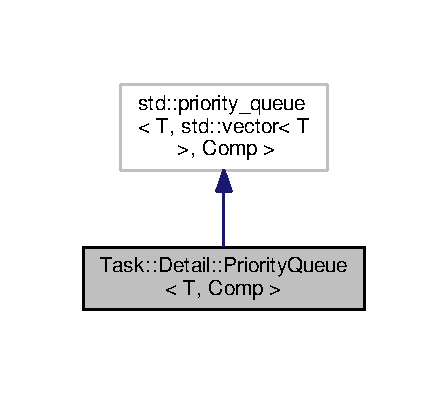
\includegraphics[width=215pt]{classTask_1_1Detail_1_1PriorityQueue__inherit__graph}
\end{center}
\end{figure}


Collaboration diagram for Task\+:\+:Detail\+:\+:Priority\+Queue$<$ T, Comp $>$\+:
\nopagebreak
\begin{figure}[H]
\begin{center}
\leavevmode
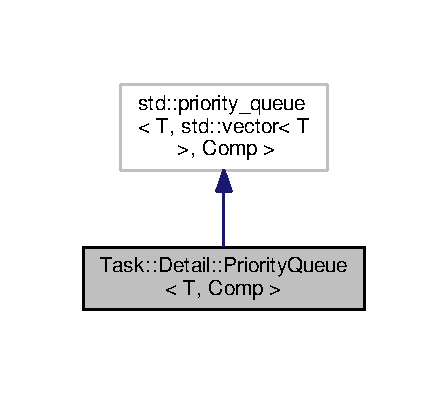
\includegraphics[width=215pt]{classTask_1_1Detail_1_1PriorityQueue__coll__graph}
\end{center}
\end{figure}
\subsection*{Public Member Functions}
\begin{DoxyCompactItemize}
\item 
\mbox{\Hypertarget{classTask_1_1Detail_1_1PriorityQueue_aa5659e1b7c5ca7b03421973ddb515c50}\label{classTask_1_1Detail_1_1PriorityQueue_aa5659e1b7c5ca7b03421973ddb515c50}} 
bool {\bfseries erase} (const T \&e)
\item 
\mbox{\Hypertarget{classTask_1_1Detail_1_1PriorityQueue_ad151f63dfc6b3f233fdc32d1e9cefc90}\label{classTask_1_1Detail_1_1PriorityQueue_ad151f63dfc6b3f233fdc32d1e9cefc90}} 
bool {\bfseries update} (const T \&e)
\item 
\mbox{\Hypertarget{classTask_1_1Detail_1_1PriorityQueue_a577cce55fe45052da1392e15db1431e4}\label{classTask_1_1Detail_1_1PriorityQueue_a577cce55fe45052da1392e15db1431e4}} 
bool {\bfseries contain} (const T \&e) const
\item 
\mbox{\Hypertarget{classTask_1_1Detail_1_1PriorityQueue_abbcbc1fe4e627576428e5d63ac565cec}\label{classTask_1_1Detail_1_1PriorityQueue_abbcbc1fe4e627576428e5d63ac565cec}} 
void {\bfseries clear} ()
\end{DoxyCompactItemize}


The documentation for this class was generated from the following file\+:\begin{DoxyCompactItemize}
\item 
include/\+Task\+Manager/detail/Priority\+Queue.\+hpp\end{DoxyCompactItemize}

\hypertarget{classTask_1_1Scheduler}{}\section{Task\+:\+:Scheduler Class Reference}
\label{classTask_1_1Scheduler}\index{Task\+::\+Scheduler@{Task\+::\+Scheduler}}


The task scheduler.  




{\ttfamily \#include $<$Scheduler.\+hpp$>$}

\subsection*{Public Member Functions}
\begin{DoxyCompactItemize}
\item 
\hyperlink{classTask_1_1Scheduler_a5ea9aca03803b6d0ee786841b8e49759}{Scheduler} (std\+::shared\+\_\+ptr$<$ \hyperlink{classTask_1_1Detail_1_1Threadpool}{Detail\+::\+Threadpool} $>$ threadpool, size\+\_\+t max\+Workers)
\item 
std\+::future$<$ void $>$ \hyperlink{classTask_1_1Scheduler_ae8b5e676c81dc9ed81e5ff0e03830d5f}{stop} (bool discard=false)
\item 
{\footnotesize template$<$class F , class... Args$>$ }\\auto \hyperlink{classTask_1_1Scheduler_a18f292492bf81fe40dc0b2c738c675f8}{schedule\+In} (const std\+::string \&id, Duration delay, F \&\&function, Args \&\&... args)
\item 
{\footnotesize template$<$class F , class... Args$>$ }\\auto \hyperlink{classTask_1_1Scheduler_a02811a81c637db4cf27261c58e1a7060}{schedule\+At} (const std\+::string \&id, Detail\+::\+Timepoint timepoint, F \&\&function, Args \&\&... args) -\/$>$ std\+::future$<$ typename std\+::result\+\_\+of$<$ F(Args...)$>$\+::type $>$
\item 
{\footnotesize template$<$class F , class... Args$>$ }\\void \hyperlink{classTask_1_1Scheduler_a00149af09fa04110105ba575bc7e88fe}{schedule\+Every} (const std\+::string \&id, Duration delay, F \&\&function, Args \&\&... args)
\item 
void \hyperlink{classTask_1_1Scheduler_a054abc32dfe84571e2591cee11de2ab1}{remove} (const std\+::string \&id)
\item 
bool \hyperlink{classTask_1_1Scheduler_a50bb4dbf7d2d232d6ebc6a109166e4ab}{is\+Scheduled} (const std\+::string \&id) const
\end{DoxyCompactItemize}


\subsection{Detailed Description}
The task scheduler. 

\subsection{Constructor \& Destructor Documentation}
\mbox{\Hypertarget{classTask_1_1Scheduler_a5ea9aca03803b6d0ee786841b8e49759}\label{classTask_1_1Scheduler_a5ea9aca03803b6d0ee786841b8e49759}} 
\index{Task\+::\+Scheduler@{Task\+::\+Scheduler}!Scheduler@{Scheduler}}
\index{Scheduler@{Scheduler}!Task\+::\+Scheduler@{Task\+::\+Scheduler}}
\subsubsection{\texorpdfstring{Scheduler()}{Scheduler()}}
{\footnotesize\ttfamily Task\+::\+Scheduler\+::\+Scheduler (\begin{DoxyParamCaption}\item[{std\+::shared\+\_\+ptr$<$ \hyperlink{classTask_1_1Detail_1_1Threadpool}{Detail\+::\+Threadpool} $>$}]{threadpool,  }\item[{size\+\_\+t}]{max\+Workers }\end{DoxyParamCaption})}

Task scheduler constructor. 
\begin{DoxyParams}{Parameters}
{\em threadpool} & The threadpool owning the workers. \\
\hline
{\em max\+Workers} & The maximum number of parallel executions. \\
\hline
\end{DoxyParams}


\subsection{Member Function Documentation}
\mbox{\Hypertarget{classTask_1_1Scheduler_a50bb4dbf7d2d232d6ebc6a109166e4ab}\label{classTask_1_1Scheduler_a50bb4dbf7d2d232d6ebc6a109166e4ab}} 
\index{Task\+::\+Scheduler@{Task\+::\+Scheduler}!is\+Scheduled@{is\+Scheduled}}
\index{is\+Scheduled@{is\+Scheduled}!Task\+::\+Scheduler@{Task\+::\+Scheduler}}
\subsubsection{\texorpdfstring{is\+Scheduled()}{isScheduled()}}
{\footnotesize\ttfamily bool Task\+::\+Scheduler\+::is\+Scheduled (\begin{DoxyParamCaption}\item[{const std\+::string \&}]{id }\end{DoxyParamCaption}) const}

Check if a task is scheduled. 
\begin{DoxyParams}{Parameters}
{\em id} & The unique identity of the task. \\
\hline
\end{DoxyParams}
\begin{DoxyReturn}{Returns}
{\ttfamily true} if it is scheduled, {\ttfamily false} otherwise. 
\end{DoxyReturn}
\mbox{\Hypertarget{classTask_1_1Scheduler_a054abc32dfe84571e2591cee11de2ab1}\label{classTask_1_1Scheduler_a054abc32dfe84571e2591cee11de2ab1}} 
\index{Task\+::\+Scheduler@{Task\+::\+Scheduler}!remove@{remove}}
\index{remove@{remove}!Task\+::\+Scheduler@{Task\+::\+Scheduler}}
\subsubsection{\texorpdfstring{remove()}{remove()}}
{\footnotesize\ttfamily void Task\+::\+Scheduler\+::remove (\begin{DoxyParamCaption}\item[{const std\+::string \&}]{id }\end{DoxyParamCaption})}

Remove a task from the scheduler. 
\begin{DoxyParams}{Parameters}
{\em id} & The unique identity of the task. \\
\hline
\end{DoxyParams}
\mbox{\Hypertarget{classTask_1_1Scheduler_a02811a81c637db4cf27261c58e1a7060}\label{classTask_1_1Scheduler_a02811a81c637db4cf27261c58e1a7060}} 
\index{Task\+::\+Scheduler@{Task\+::\+Scheduler}!schedule\+At@{schedule\+At}}
\index{schedule\+At@{schedule\+At}!Task\+::\+Scheduler@{Task\+::\+Scheduler}}
\subsubsection{\texorpdfstring{schedule\+At()}{scheduleAt()}}
{\footnotesize\ttfamily template$<$class F , class... Args$>$ \\
auto Task\+::\+Scheduler\+::schedule\+At (\begin{DoxyParamCaption}\item[{const std\+::string \&}]{id,  }\item[{Detail\+::\+Timepoint}]{timepoint,  }\item[{F \&\&}]{function,  }\item[{Args \&\&...}]{args }\end{DoxyParamCaption}) -\/$>$ std\+::future$<$typename std\+::result\+\_\+of$<$F(Args...)$>$\+::type$>$ \hspace{0.3cm}{\ttfamily [inline]}}

Add a new task to the scheduler. 
\begin{DoxyParams}{Parameters}
{\em id} & The unique identity of the task. \\
\hline
{\em timepoint} & The timepoint to reach before executing the task. \\
\hline
{\em function} & The function to execute. \\
\hline
{\em args} & the parameters to pass to the function. \\
\hline
\end{DoxyParams}
\mbox{\Hypertarget{classTask_1_1Scheduler_a00149af09fa04110105ba575bc7e88fe}\label{classTask_1_1Scheduler_a00149af09fa04110105ba575bc7e88fe}} 
\index{Task\+::\+Scheduler@{Task\+::\+Scheduler}!schedule\+Every@{schedule\+Every}}
\index{schedule\+Every@{schedule\+Every}!Task\+::\+Scheduler@{Task\+::\+Scheduler}}
\subsubsection{\texorpdfstring{schedule\+Every()}{scheduleEvery()}}
{\footnotesize\ttfamily template$<$class F , class... Args$>$ \\
void Task\+::\+Scheduler\+::schedule\+Every (\begin{DoxyParamCaption}\item[{const std\+::string \&}]{id,  }\item[{Duration}]{delay,  }\item[{F \&\&}]{function,  }\item[{Args \&\&...}]{args }\end{DoxyParamCaption})\hspace{0.3cm}{\ttfamily [inline]}}

Add a new periodic task to the scheduler. 
\begin{DoxyParams}{Parameters}
{\em id} & The unique identity of the task. \\
\hline
{\em delay} & The minimum duration separating two executions. \\
\hline
{\em function} & The function to execute. \\
\hline
{\em args} & the parameters to pass to the function. \\
\hline
\end{DoxyParams}
\mbox{\Hypertarget{classTask_1_1Scheduler_a18f292492bf81fe40dc0b2c738c675f8}\label{classTask_1_1Scheduler_a18f292492bf81fe40dc0b2c738c675f8}} 
\index{Task\+::\+Scheduler@{Task\+::\+Scheduler}!schedule\+In@{schedule\+In}}
\index{schedule\+In@{schedule\+In}!Task\+::\+Scheduler@{Task\+::\+Scheduler}}
\subsubsection{\texorpdfstring{schedule\+In()}{scheduleIn()}}
{\footnotesize\ttfamily template$<$class F , class... Args$>$ \\
auto Task\+::\+Scheduler\+::schedule\+In (\begin{DoxyParamCaption}\item[{const std\+::string \&}]{id,  }\item[{Duration}]{delay,  }\item[{F \&\&}]{function,  }\item[{Args \&\&...}]{args }\end{DoxyParamCaption})\hspace{0.3cm}{\ttfamily [inline]}}

Add a new task to the scheduler. 
\begin{DoxyParams}{Parameters}
{\em id} & The unique identity of the task. \\
\hline
{\em delay} & The delay to wait before executing the task. \\
\hline
{\em function} & The function to execute. \\
\hline
{\em args} & the parameters to pass to the function. \\
\hline
\end{DoxyParams}
\mbox{\Hypertarget{classTask_1_1Scheduler_ae8b5e676c81dc9ed81e5ff0e03830d5f}\label{classTask_1_1Scheduler_ae8b5e676c81dc9ed81e5ff0e03830d5f}} 
\index{Task\+::\+Scheduler@{Task\+::\+Scheduler}!stop@{stop}}
\index{stop@{stop}!Task\+::\+Scheduler@{Task\+::\+Scheduler}}
\subsubsection{\texorpdfstring{stop()}{stop()}}
{\footnotesize\ttfamily std\+::future$<$void$>$ Task\+::\+Scheduler\+::stop (\begin{DoxyParamCaption}\item[{bool}]{discard = {\ttfamily false} }\end{DoxyParamCaption})}

Synchronize and stop the task scheduler. 
\begin{DoxyParams}{Parameters}
{\em discard} & {\ttfamily true} Discard the tasks scheduled for the future. \\
\hline
\end{DoxyParams}
\begin{DoxyReturn}{Returns}
A future that signals when the scheduler can be destroyed. 
\end{DoxyReturn}


The documentation for this class was generated from the following file\+:\begin{DoxyCompactItemize}
\item 
include/\+Task\+Manager/Scheduler.\+hpp\end{DoxyCompactItemize}

\hypertarget{classTask_1_1Detail_1_1Threadpool}{}\section{Task\+:\+:Detail\+:\+:Threadpool Class Reference}
\label{classTask_1_1Detail_1_1Threadpool}\index{Task\+::\+Detail\+::\+Threadpool@{Task\+::\+Detail\+::\+Threadpool}}
\subsection*{Public Member Functions}
\begin{DoxyCompactItemize}
\item 
\mbox{\Hypertarget{classTask_1_1Detail_1_1Threadpool_aeb9a8c7ee6d72b9fa7294eb86340f133}\label{classTask_1_1Detail_1_1Threadpool_aeb9a8c7ee6d72b9fa7294eb86340f133}} 
{\bfseries Threadpool} (size\+\_\+t thread\+Count)
\item 
\mbox{\Hypertarget{classTask_1_1Detail_1_1Threadpool_a11897665b92483387fa1b5eb2b719b48}\label{classTask_1_1Detail_1_1Threadpool_a11897665b92483387fa1b5eb2b719b48}} 
void {\bfseries execute} (\hyperlink{classTask_1_1Detail_1_1TimedTask}{Timed\+Task} task)
\end{DoxyCompactItemize}


The documentation for this class was generated from the following file\+:\begin{DoxyCompactItemize}
\item 
include/\+Task\+Manager/detail/Threadpool.\+hpp\end{DoxyCompactItemize}

\hypertarget{classTask_1_1Detail_1_1TimedTask}{}\section{Task\+:\+:Detail\+:\+:Timed\+Task Class Reference}
\label{classTask_1_1Detail_1_1TimedTask}\index{Task\+::\+Detail\+::\+Timed\+Task@{Task\+::\+Detail\+::\+Timed\+Task}}
\subsection*{Public Member Functions}
\begin{DoxyCompactItemize}
\item 
\mbox{\Hypertarget{classTask_1_1Detail_1_1TimedTask_a08d21b8047bf71739948ac70ba6013a9}\label{classTask_1_1Detail_1_1TimedTask_a08d21b8047bf71739948ac70ba6013a9}} 
{\bfseries Timed\+Task} (Task functor, const Timepoint \&timepoint)
\item 
\mbox{\Hypertarget{classTask_1_1Detail_1_1TimedTask_aa978842dfcd5984db8133cf5d54a9f56}\label{classTask_1_1Detail_1_1TimedTask_aa978842dfcd5984db8133cf5d54a9f56}} 
const Timepoint \& {\bfseries timepoint} () const
\item 
\mbox{\Hypertarget{classTask_1_1Detail_1_1TimedTask_a2a256f1f655755dc45e4693114dfe82b}\label{classTask_1_1Detail_1_1TimedTask_a2a256f1f655755dc45e4693114dfe82b}} 
bool {\bfseries operator$>$} (const \hyperlink{classTask_1_1Detail_1_1TimedTask}{Timed\+Task} \&other) const
\item 
\mbox{\Hypertarget{classTask_1_1Detail_1_1TimedTask_a6915f45e065ac53ea328b8bff29dc3ba}\label{classTask_1_1Detail_1_1TimedTask_a6915f45e065ac53ea328b8bff29dc3ba}} 
void {\bfseries operator()} ()
\end{DoxyCompactItemize}


The documentation for this class was generated from the following file\+:\begin{DoxyCompactItemize}
\item 
include/\+Task\+Manager/detail/Task.\+hpp\end{DoxyCompactItemize}

%--- End generated contents ---

% Index
\backmatter
\newpage
\phantomsection
\clearemptydoublepage
\addcontentsline{toc}{chapter}{Index}
\printindex

\end{document}
